\section{Aufbau und Durchführung}

\subsection{Aufbau}
\label{subsec:Aufbau}
Der verwendete Versuchsaufbau ist in \autoref{pic:Aufbau_Foto} zu sehen. Grundlegend für den Versuch ist der Rezipient, der die Probe in einem Vakuum hält. Das Vakuum wird dauerhaft durch eine Vakuumpumpe aufrecht erhalten und mithilfe eines Pirani-Vakuummeter gemessen. Als Probe wird mit Strontium dotiertes Kaliumbromid verwendet. Diese ist innerhalb des Rezipient auf den Boden aufgekittet, wie in \autoref{pic:Rezipient_Foto} zu sehen. Auf der Probe ist eine Metallplatte angebracht, sodass zwischen Boden und Metallplatte eine Spannung mithilfe des Spannungsgenerators angelegt werden kann. An dem Plattenkondensator liegt außerdem das Amperemeter an. Der Boden des Rezipienten ist außerdem mit dem Kühlfinger verbunden, der in ein Dewargefäß reicht, welches mit flüssigem Stickstoff gefüllt werden kann. Das Dewargefäß steht auf einem höhenverstellbaren Tisch. Die Probe kann außerdem mithilfe einer Heizwickel erhitzt werden.
%\begin{figure}
%    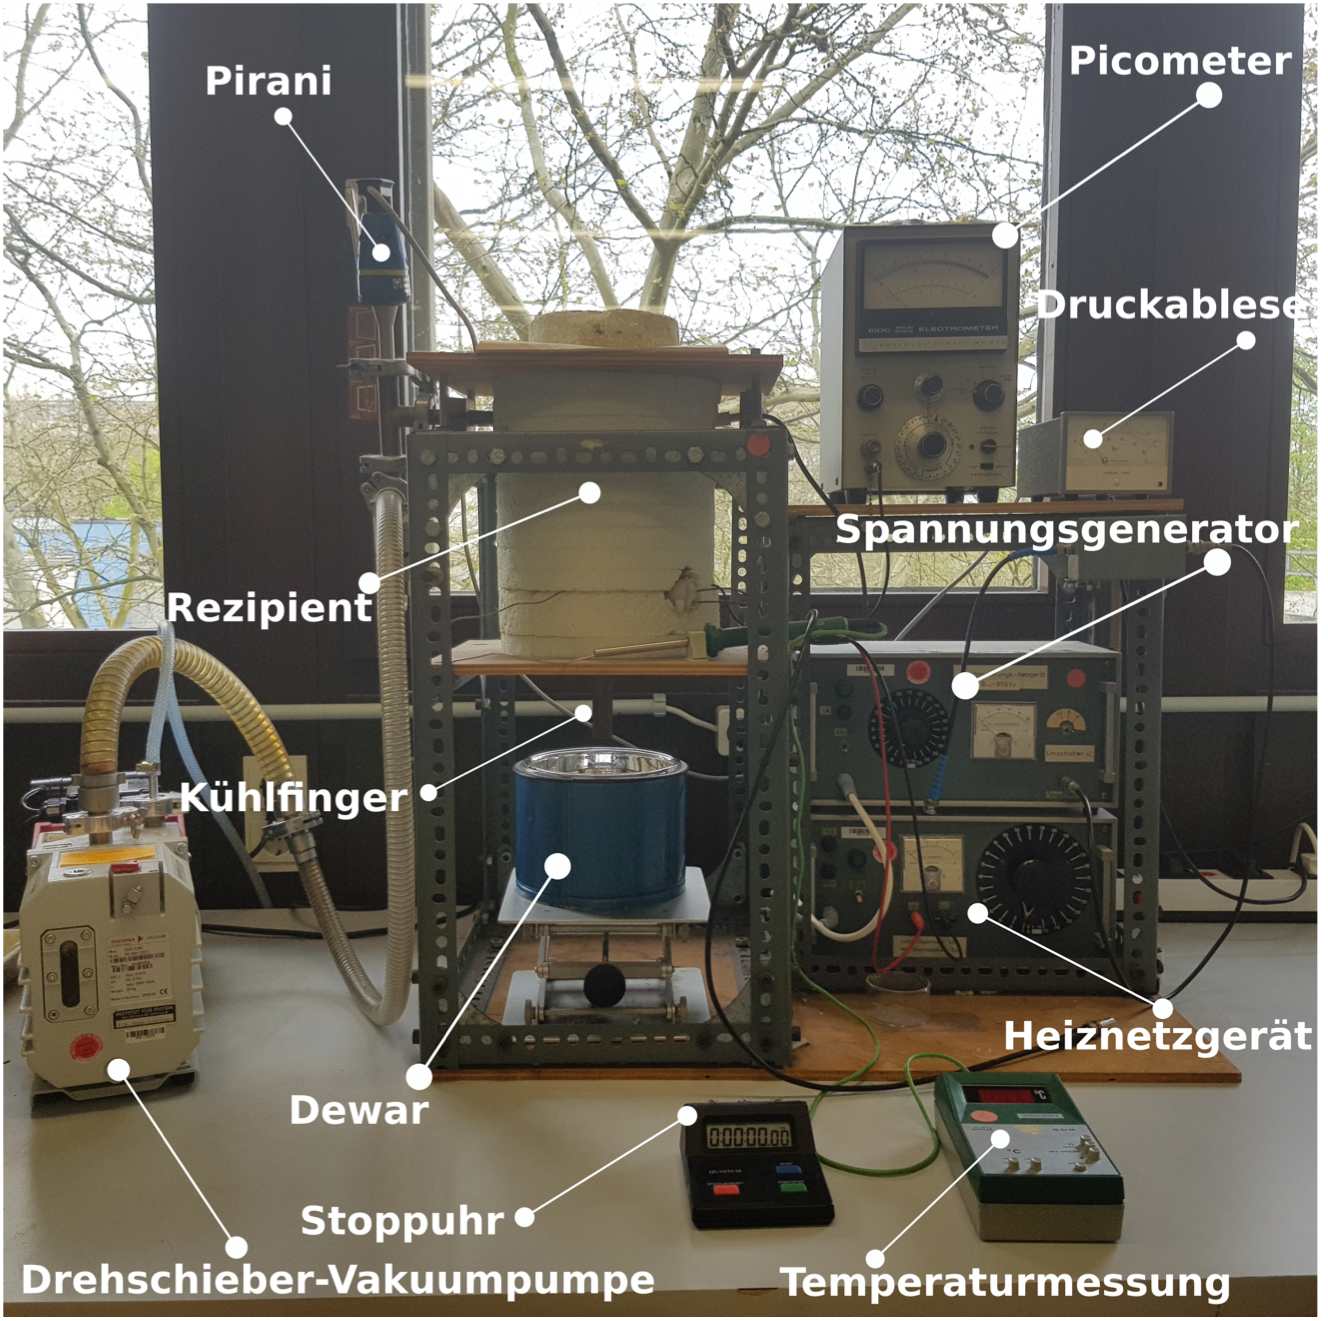
\includegraphics[width=0.45\linewidth]{Bilder/Aufbau.jpeg}
%    \caption{Foto des Versuchsaufbaus mit Beschriftung der Bestandteile.\cite{anleitungV48}}
%    \label{pic:Aufbau_Foto}
%    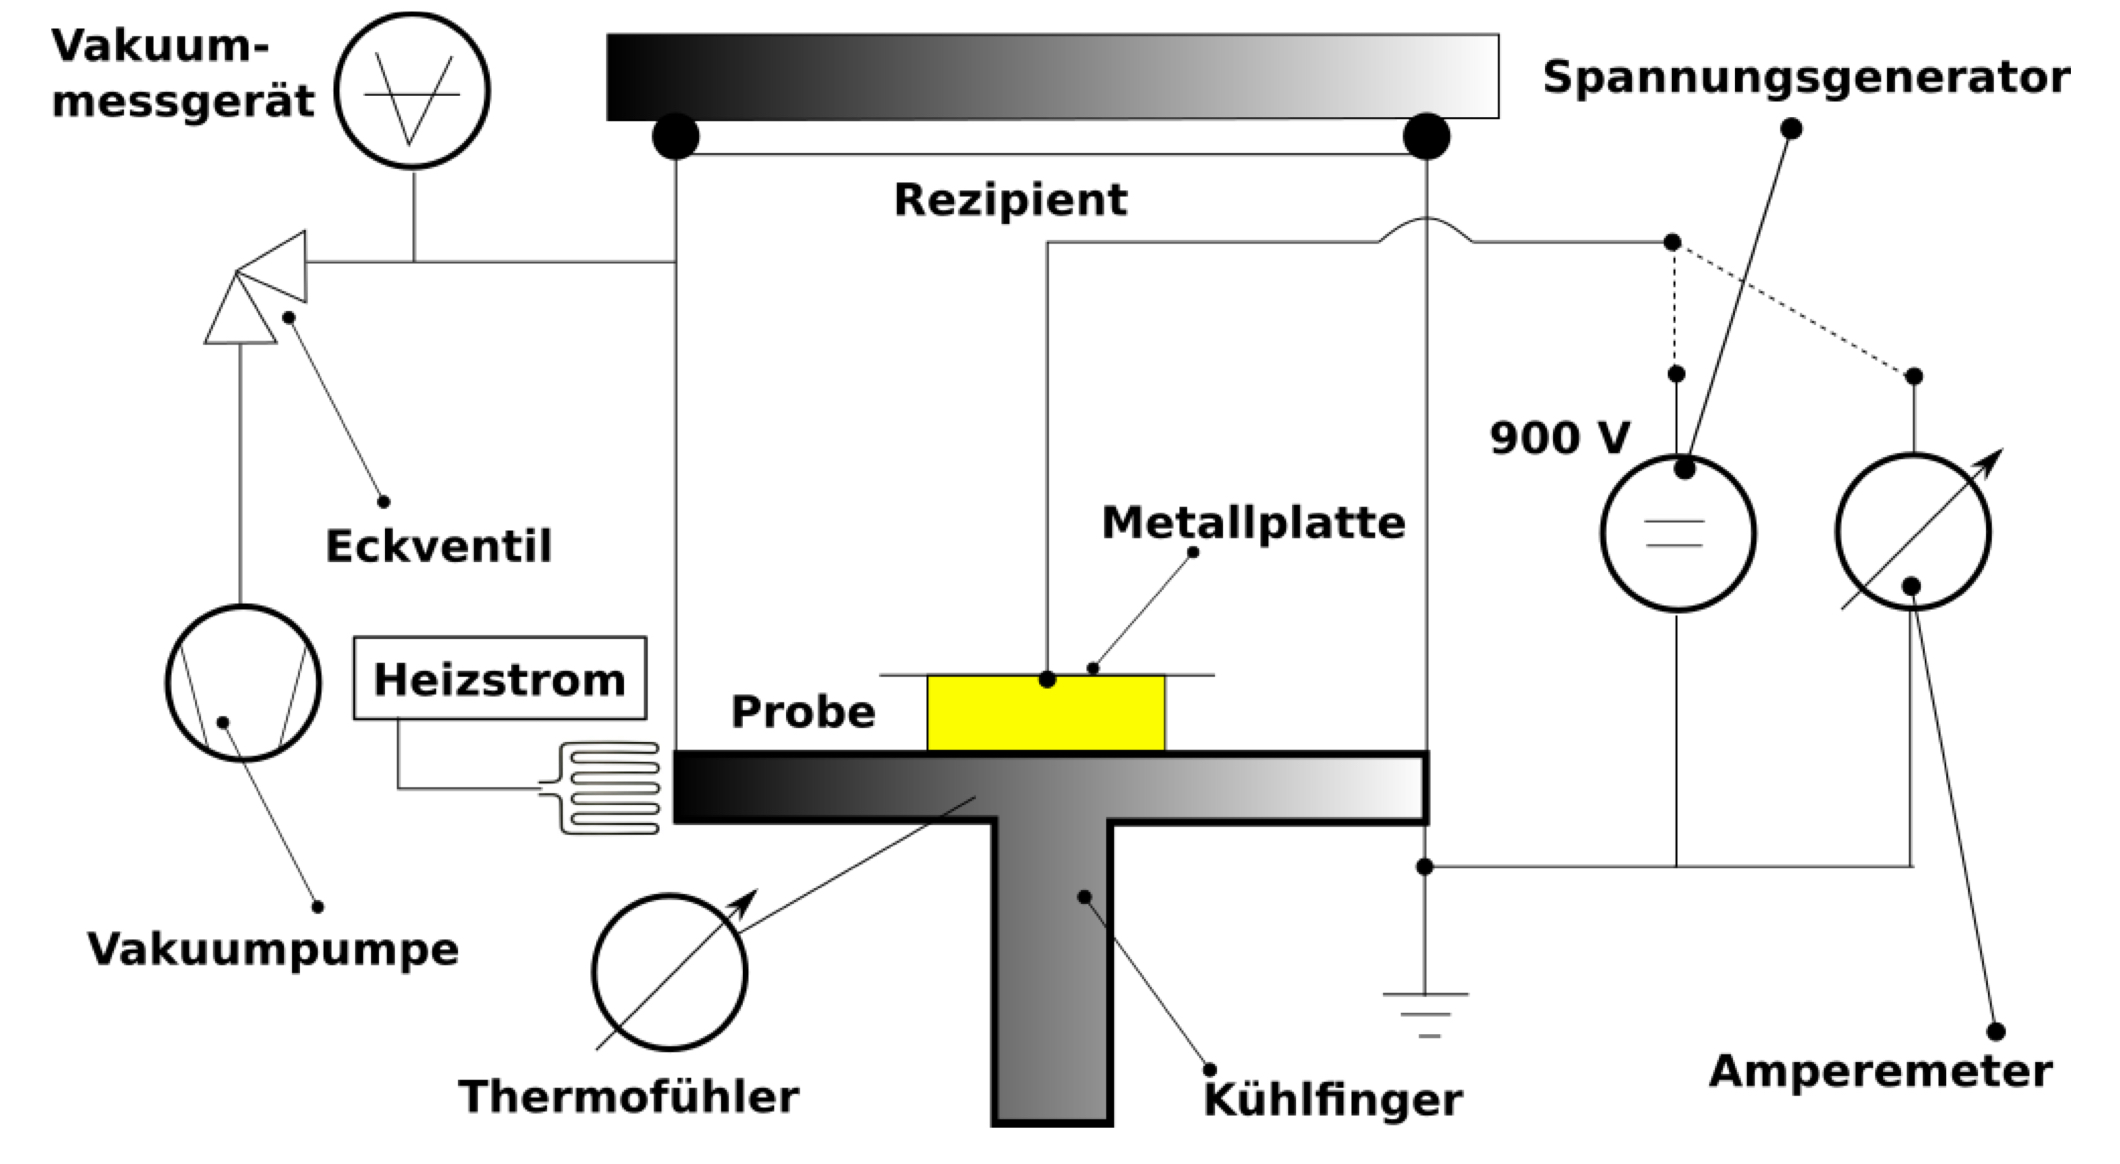
\includegraphics[width=0.45\linewidth]{Bilder/Rezipient.jpeg}
%    \caption{Schematische Darstellung des Rezipienten und anliegender Messtechnik.\cite{anleitungV48}}
%    \label{pic:Rezipient_Foto}
%\end{figure}

\begin{figure}
    \centering
    \begin{subfigure}[t]{0.5\linewidth}
        \centering
        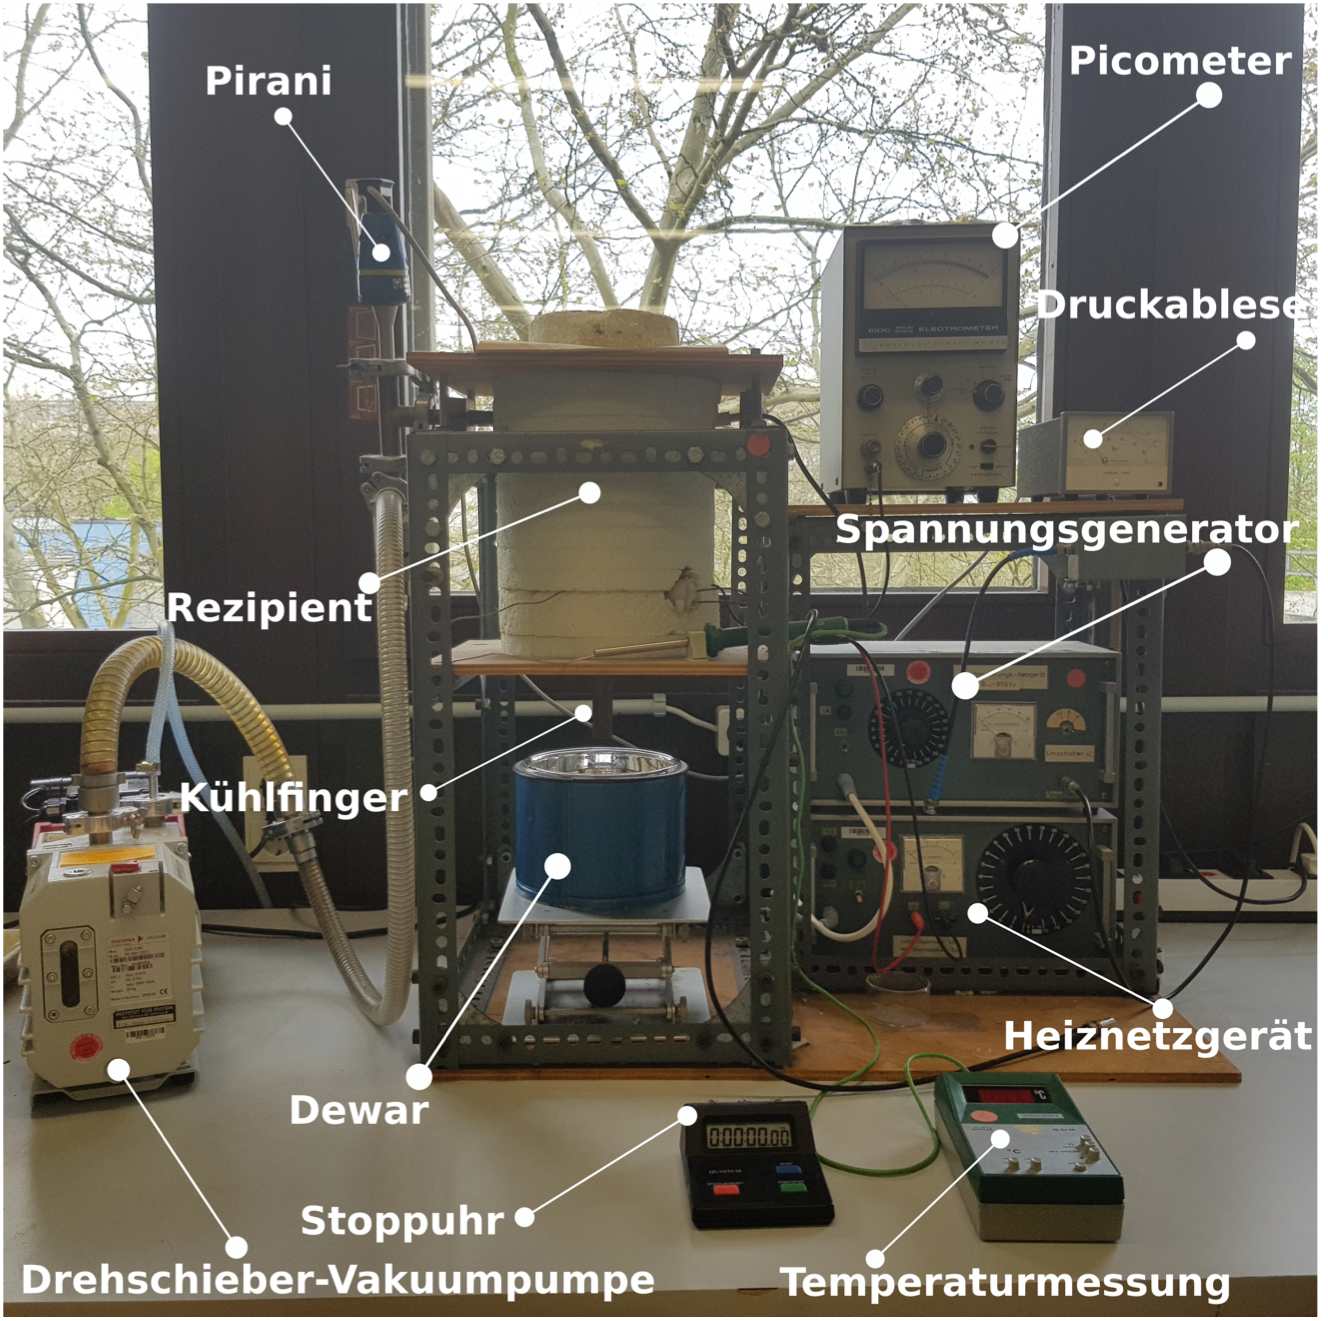
\includegraphics[width=\linewidth]{Bilder/Aufbau.jpeg}
        \caption{Foto des Versuchsaufbaus mit Beschriftung der Bestandteile.}
        \label{pic:Aufbau_Foto}
    \end{subfigure}%
    ~ 
    \begin{subfigure}[t]{0.5\linewidth}
        \centering
        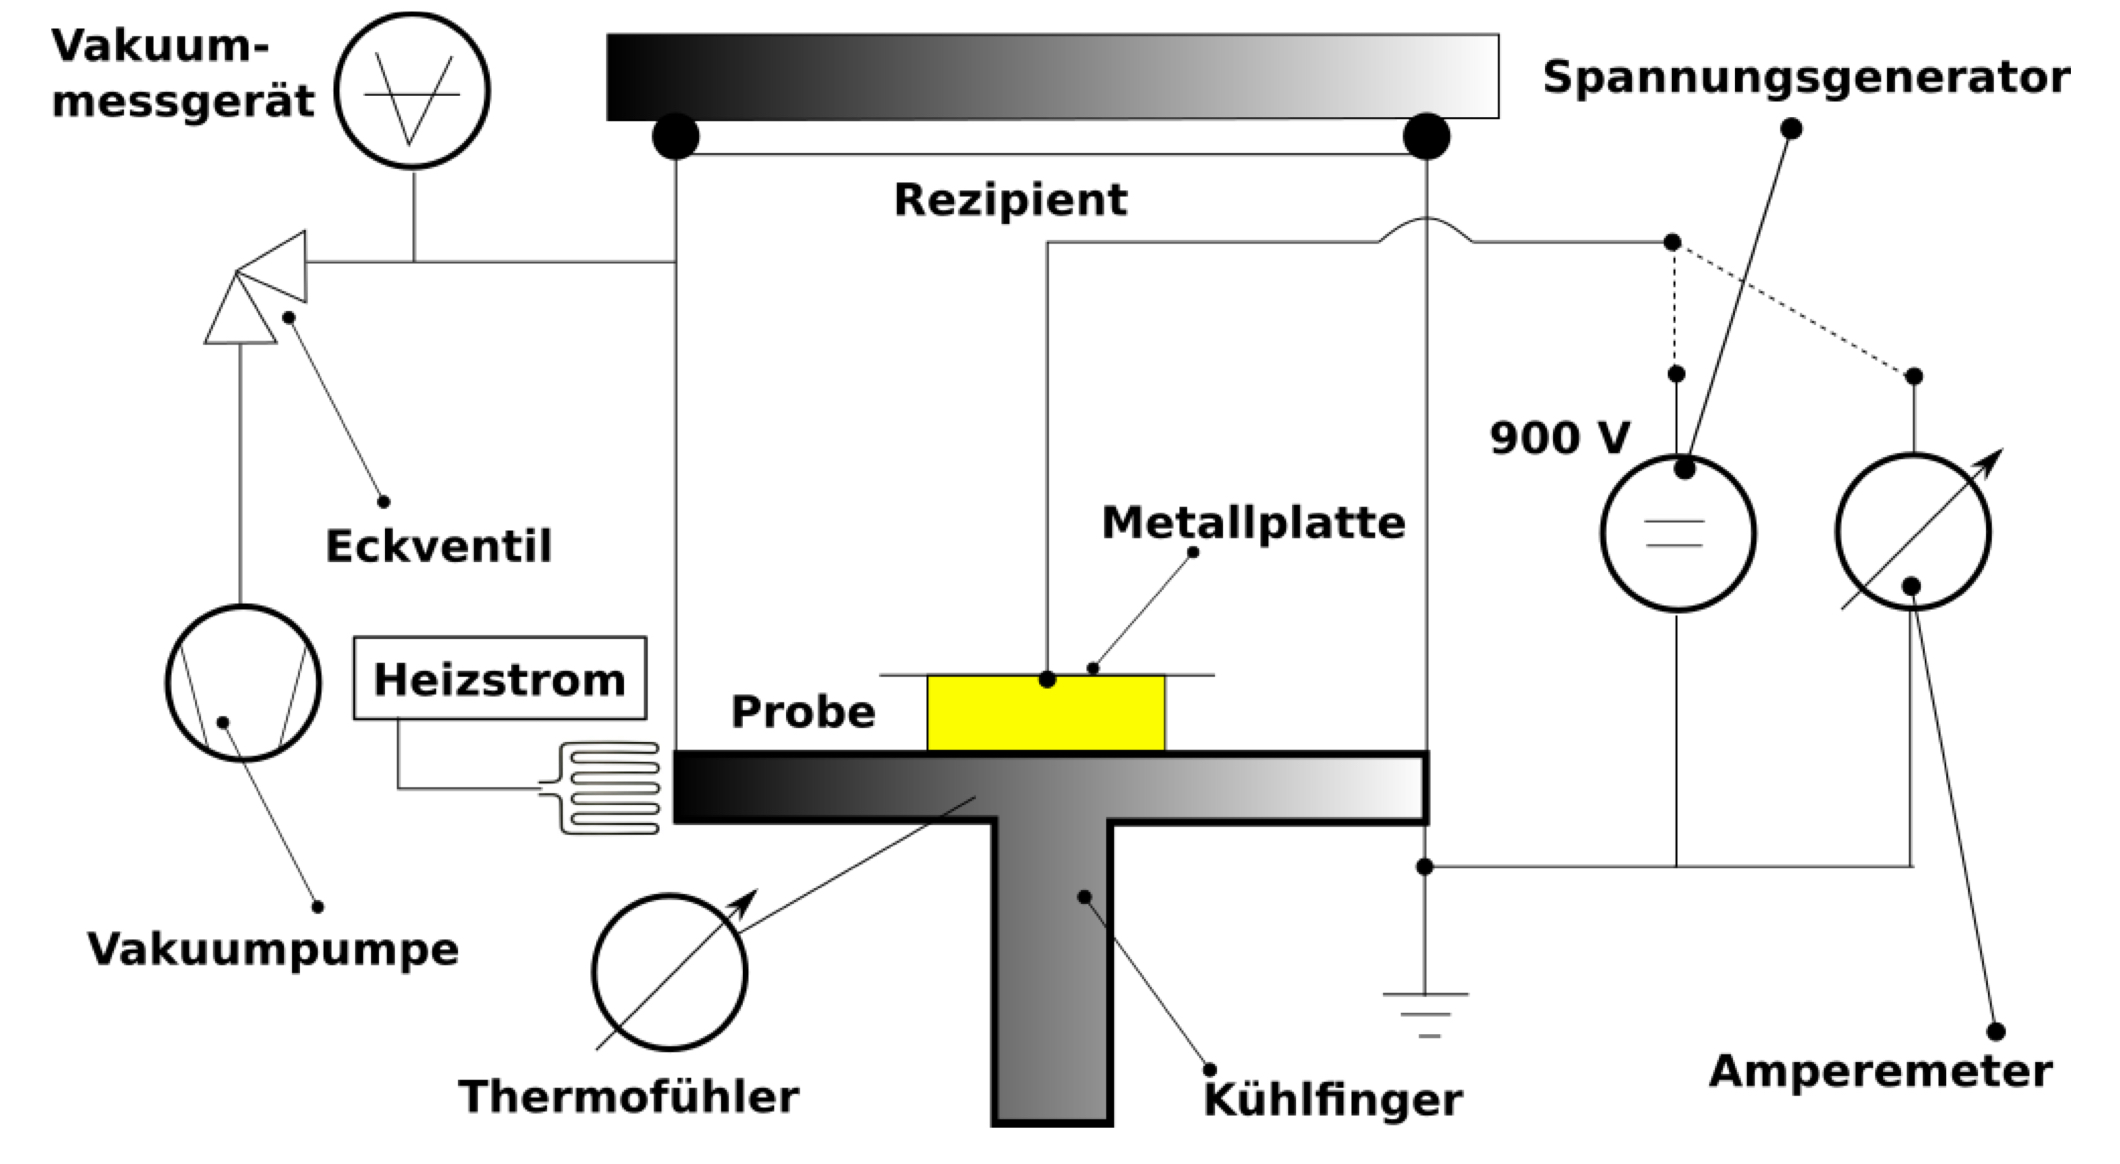
\includegraphics[width=\linewidth]{Bilder/Rezipient.jpeg}
        \caption{Schematische Darstellung des Rezipienten und anliegender Messtechnik.}
        \label{pic:Rezipient_Foto}
    \end{subfigure}
    \caption{Versuchsaufbau der Ionen-Thermostrom-Methode.\cite{anleitungV48}}
    \label{pic:Gesamter_Versuchsaufbau}
\end{figure}
\FloatBarrier

\subsection{Durchführung}
\label{subsec:Durchführung}
Zu Beginn wird die Probe auf über $45 \, ° \symup{C}$ erhitzt. Dann wird der Plattenkondensator auf $950 \, \unit{\volt}$ aufgeladen und die Spannung für mindestens $15 \, \unit{\minute}$ aufrecht gehalten. Anschließend wird flüssiger Stickstoff in das Dewargefäß gefüllt und die Probe auf $-60 \, ° \symup{C}$ gekühlt. Nach Erreichen der Temperatur wird das elektrische Feld ausgeschaltet und der Plattenkondensator durch  $15 \, \unit{\minute}$ kurzschließen entladen. Anschließend wird das Amperemeter angeschlossen und bei konstanter Heizrate der Strom und die Temperatur jede Minute notiert. Diese gesamte Durchführung wird noch einmal wiederholt bei einer anderen Heizrate. Es werden Heizraten von ungefähr $1,5 \, \frac{° \symup{C}}{\unit{\minute}}$ und $2 \, \frac{° \symup{C}}{\unit{\minute}}$ angestrebt.